\documentclass[conference]{IEEEtran}
\IEEEoverridecommandlockouts
% The preceding line is only needed to identify funding in the first footnote. If that is unneeded, please comment it out.
\usepackage{cite}
\usepackage{amsmath,amssymb,amsfonts}
\usepackage{algorithmic}
\usepackage{graphicx}
\usepackage{textcomp}
\usepackage{xcolor}
\usepackage{hyperref} % Add this line
\def\BibTeX{{\rm B\kern-.05em{\sc i\kern-.025em b}\kern-.08em
    T\kern-.1667em\lower.7ex\hbox{E}\kern-.125emX}}
\begin{document}

\title{Not Quite My Tempo: Symbolic Music Generation With Mamba Architecture}

\author{\IEEEauthorblockN{Jan Retkowski}
    \IEEEauthorblockA{
        % \textit{Faculty of Electronics and Information Technology} \\
        % \textit{Warsaw University of Technology}\\
        % Warsaw, Poland \\
        TODO@gmail.com}
    \and
    \IEEEauthorblockN{Milosz Lopatto}
    \IEEEauthorblockA{
        TODO@gmail.com\\
        \textit{Faculty of Electronics and Information Technology} \\
        \textit{Warsaw University of Technology}\\
        Warsaw, Poland}
    \and
    \IEEEauthorblockN{Jakub Stepniak}
    \IEEEauthorblockA{
        % \textit{Faculty of Electronics and Information Technology} \\
        % \textit{Warsaw University of Technology}\\
        % Warsaw, Poland \\
        TODO@gmail.com}
}

\maketitle

\begin{abstract}
    Over the past few years, a lot of effort has been put into making Transformers more and more efficient. However, they still suffer from quadratic memory and inference time complexity. Recently they have been experiencing increasing competition from state space models (SSMs), that avoid some of transformer's drawbacks. In this paper we test one of state-of-the-art SSM models called Mamba in symbolic music generation. To achieve this we conducted several experiments on MAESTRO MIDI dataset. Our results show that while mamba can be used to generate novel musical scores, their quality leaves much to be desired.
\end{abstract}

\begin{IEEEkeywords}
    deep learning, transformer, music, symbolic music generation, neural network, generative, unsupervised learning, state space model, ssm, mamba
\end{IEEEkeywords}

\section{Introduction}
% no \IEEEPARstart
Symbolic music generation has been an area of active research over the past decades. In the beginning it was dominated by classical methods like Hidden Markov Models. During the advent of deep learning in the last decade, neural networks managed to become a go-to method for this task. During those years a lot of architectures, including Long Short-term Memory networks (LSTMs) \cite{lstm}, Variational Autoencoders (VAEs) \cite{kingma2022autoencoding} and Generative Adversarial Networks (GANs) \cite{goodfellow2014generative} were used to successfully generate music in symbolic formats. However, after popularisation of Transformers \cite{attention-is-all-you-need} and Diffusion Models \cite{ho2020denoising} in the field broad of deep learning, they seem to be gaining more and more dominance in the area of symbolic music generation.  In the case of transformers, which are the go-to architecture in the area of natural language processing, a lot of effort has been put into small iterative improvements, to make them more efficient. However, they still suffer from quadratic GPU memory and inference time complexity. To mitigate those problems State Space Models (SSMs) \cite{ssm} were developed.  Recently, they have been gaining popularity and even beating transformers on some of their most signature tasks in the field of natural language processing, while being significantly smaller \cite{mamba}. They seem to be especially suited for long time dependencies. Musical data, which often contains such long dependencies, seem to be suited for further testing the performance of SSMs. Therefore we decided to use current state-of-the-art SSM model called Mamba \cite{mamba} to generate music in symbolic format.

\section{Data}
We decided to use MIDI \cite{midi} music representation. It is by far the most popular format in the field of symbolic music and allows us to freely use the largest symbolic music datasets available. Because of the model's size, a lot of data is required to reduce the chance of overfitting. The dataset we chose is MAESTRO (MIDI and Audio Edited for Synchronous TRacks and Organization) \cite{maestro1} \cite{maestro2}. It contains over 200 hours of virtuosic piano performances. The data comes from ten years of the International Piano-e-Competition. It is one of the most popular datasets, allowing us to easily compare our results to other models. The data was downloaded using Muspy \cite{muspy} library, which allows for convenient handling of symbolic musical data. Tokenization was conducted using the miditok \cite{miditok2021} library. It contains methods for tokenising MIDI data into most of the most popular formats. We decided to opt for REMI \cite{remi} format with learned Byte-Pair Encodings.

\section{Architecture}
Mamba utilises a novel approach called selective state space models (SSMs), which enhance traditional state space models by allowing
parameters to be functions of the input. This design enables the model to selectively propagate or forget information along the sequence length,
dependent on the current input token. Mamba integrates this selective SSM approach into a simplified end-to-end architecture, foregoing traditional components
like attention or MLP blocks found in architectures like Transformers.

The main difference between Selective SSM and traditional SSM is the input-dependence, which mimics what the attention mechanism in Transformers
does—essentially assessing whether a specific token is important or not. However, this feature sacrifices the ability of traditional SSMs
to precompute all learnable matrices ($\Delta$, A, B, C) and their configurations based on sequence length in a single inference pass.
To address this, we introduce a mechanism of Parallel Associative Scan (similar to Prefix Sum) that requires storing precomputed calculations,
leading to higher memory usage but still maintaining linear computation.

\begin{figure}[!htbp]
    \centering 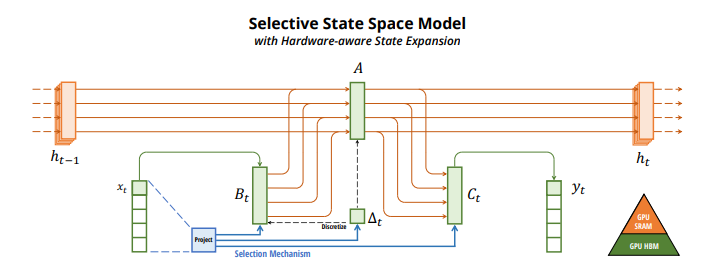
\includegraphics[width=\linewidth]{../assets/SelectiveSSM.png}
    \caption{Selective SSM \cite{mamba}}
    \label{fig:ssm}
\end{figure}

To enhance efficiency further, the authors proposed using a hardware-aware algorithm that leverages two main types of GPU memory:
SRAM, which is fast but has limited capacity (ideal for matrix calculations), and HBM, which is slower but has a larger capacity.
The main bottleneck of this approach is managing the data transfer between these memory types.

\begin{figure}[!htbp]
    \centering 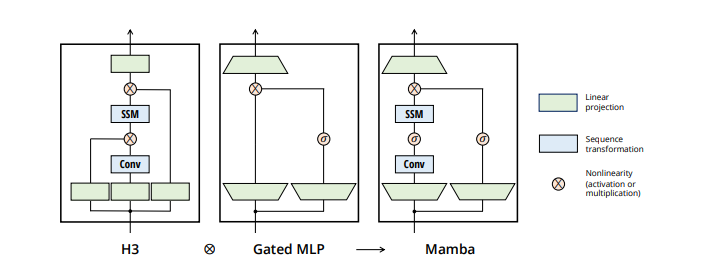
\includegraphics[width=\linewidth]{../assets/Mamba.png}
    \caption{Mamba block \cite{mamba}}
    \label{fig:mamba}
\end{figure}

Selective SSM is a crucial component of the Mamba block, but the system also includes linear layers that increase dimensionality, nonlinear layers, and gating connections.
The whole architecture is built from many Mamba blocks, which are computed layer by layer.


\begin{table}[t] \centering
    % Podpis tabeli umieszczamy od góry
    \caption{Model comparison \cite{mamba}}
    \label{tab:comparison}

    % Tabela z trzema kolumnami:
    % dwie wyrównanie do środka [c], a ostatnia do prawej [r]
    % szerokość kolumn automatyczna (równa szerokości tekstu)
    \resizebox{\linewidth}{!}{\begin{tabular}{| c | c | c | c |} \hline
            Architecture          & Complexity & Memory   & Performance \\ \hline\hline
            Transformer           & $ O(N^2)$  & $O(N^2)$ & great       \\ \hline
            RNN                   & $O(N)$     & $O(N)$   & poor        \\ \hline
            SSM                   & $O(N)$     & $O(N)$   & poor        \\ \hline
            Selective SSM (Mamba) & $O(N)$     & $O(N)$   & great.      \\ \hline
            % Komórka o szerokości dwóch kolumn, wyrównana do prawej
            % Przypisy dolne w tabelach wstawiamy przez \tablefootnote
            % \multicolumn{2}{|r|}{Suma\tablefootnote{Table footnote.}} & 123,45 \\ \hline
        \end{tabular}}
\end{table}

\begin{figure}[!htbp]
    \centering 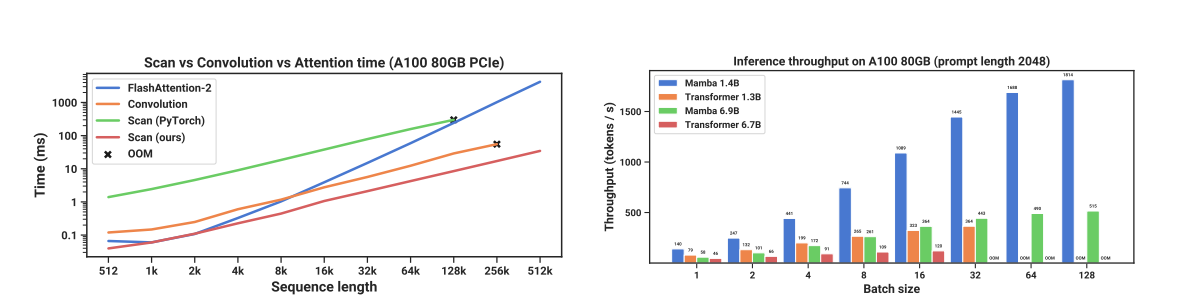
\includegraphics[width=\linewidth]{../assets/results.png}
    \caption{Benchmarks \cite{mamba}}
    \label{fig:mamba}
\end{figure}

\section{Experiments}
\subsection{Synthetic Data}
To first check that our training setup is correct, we decided to overfit the model to synthetic data. For this purpose, we generated sequence $0, 1, ..., 1999$ then tried to make the model recreate it after receiving the 0 token as input. During the training, the loss quickly approached zero. When testing the model, it managed to generate the entire sequence correctly, albeit it required tuning the generation function's parameters.

\begin{figure}[!htbp]
    \centering 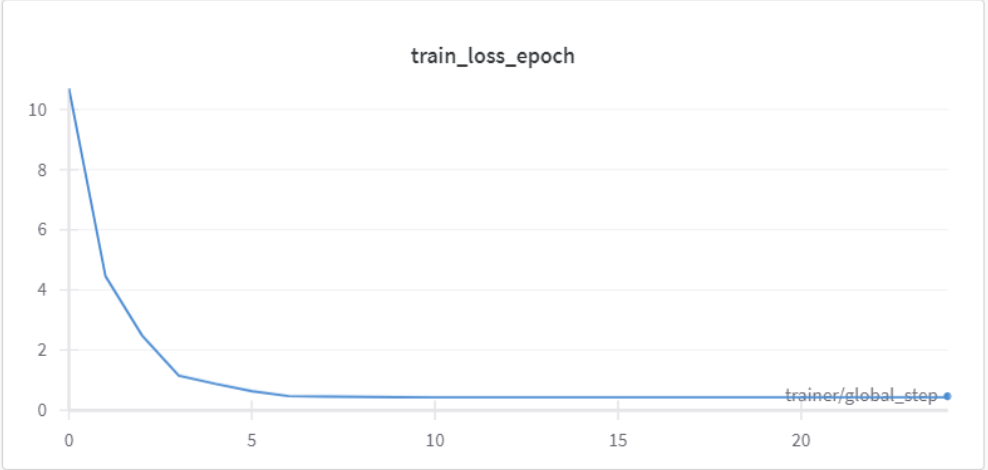
\includegraphics[width=\linewidth]{../assets/synth_data_train.png}
    \caption{ Loss during training on synthetic data}
    \label{fig:synth}
\end{figure}

We conducted a series of experiments to evaluate the performance of the Mamba architecture in symbolic music generation. The experiments are outlined as follows:

\begin{enumerate}
    \item \textbf{Simple Sequence Training}: We began by training the model on a simple numerical sequence (e.g., 0, 1, 2, 3, 4, ...). This experiment was designed to verify the model's ability to learn and reproduce basic patterns. The main goal of this part was to catch any implementation bugs as soon as possible.

    \item \textbf{Single Musical Piece Training}: Next, we trained the model on a single musical piece. This experiment aimed to assess the model's capacity to understand and generate music from a limited dataset. Even though it may seem to be a trivial task, playing with configuration was necessary – both training and inference.

    \item \textbf{Comprehensive Training on Multiple Pieces}: Finally, we conducted full-scale training using a diverse set of musical pieces from the MAESTRO dataset. This experiment was intended to evaluate the model's performance in generating complex and varied musical compositions.
\end{enumerate}

Each experiment was carefully monitored, and the generated outputs were analyzed to determine the model's effectiveness in capturing musical structures and patterns.

\begin{figure}[!htbp]
    \centering 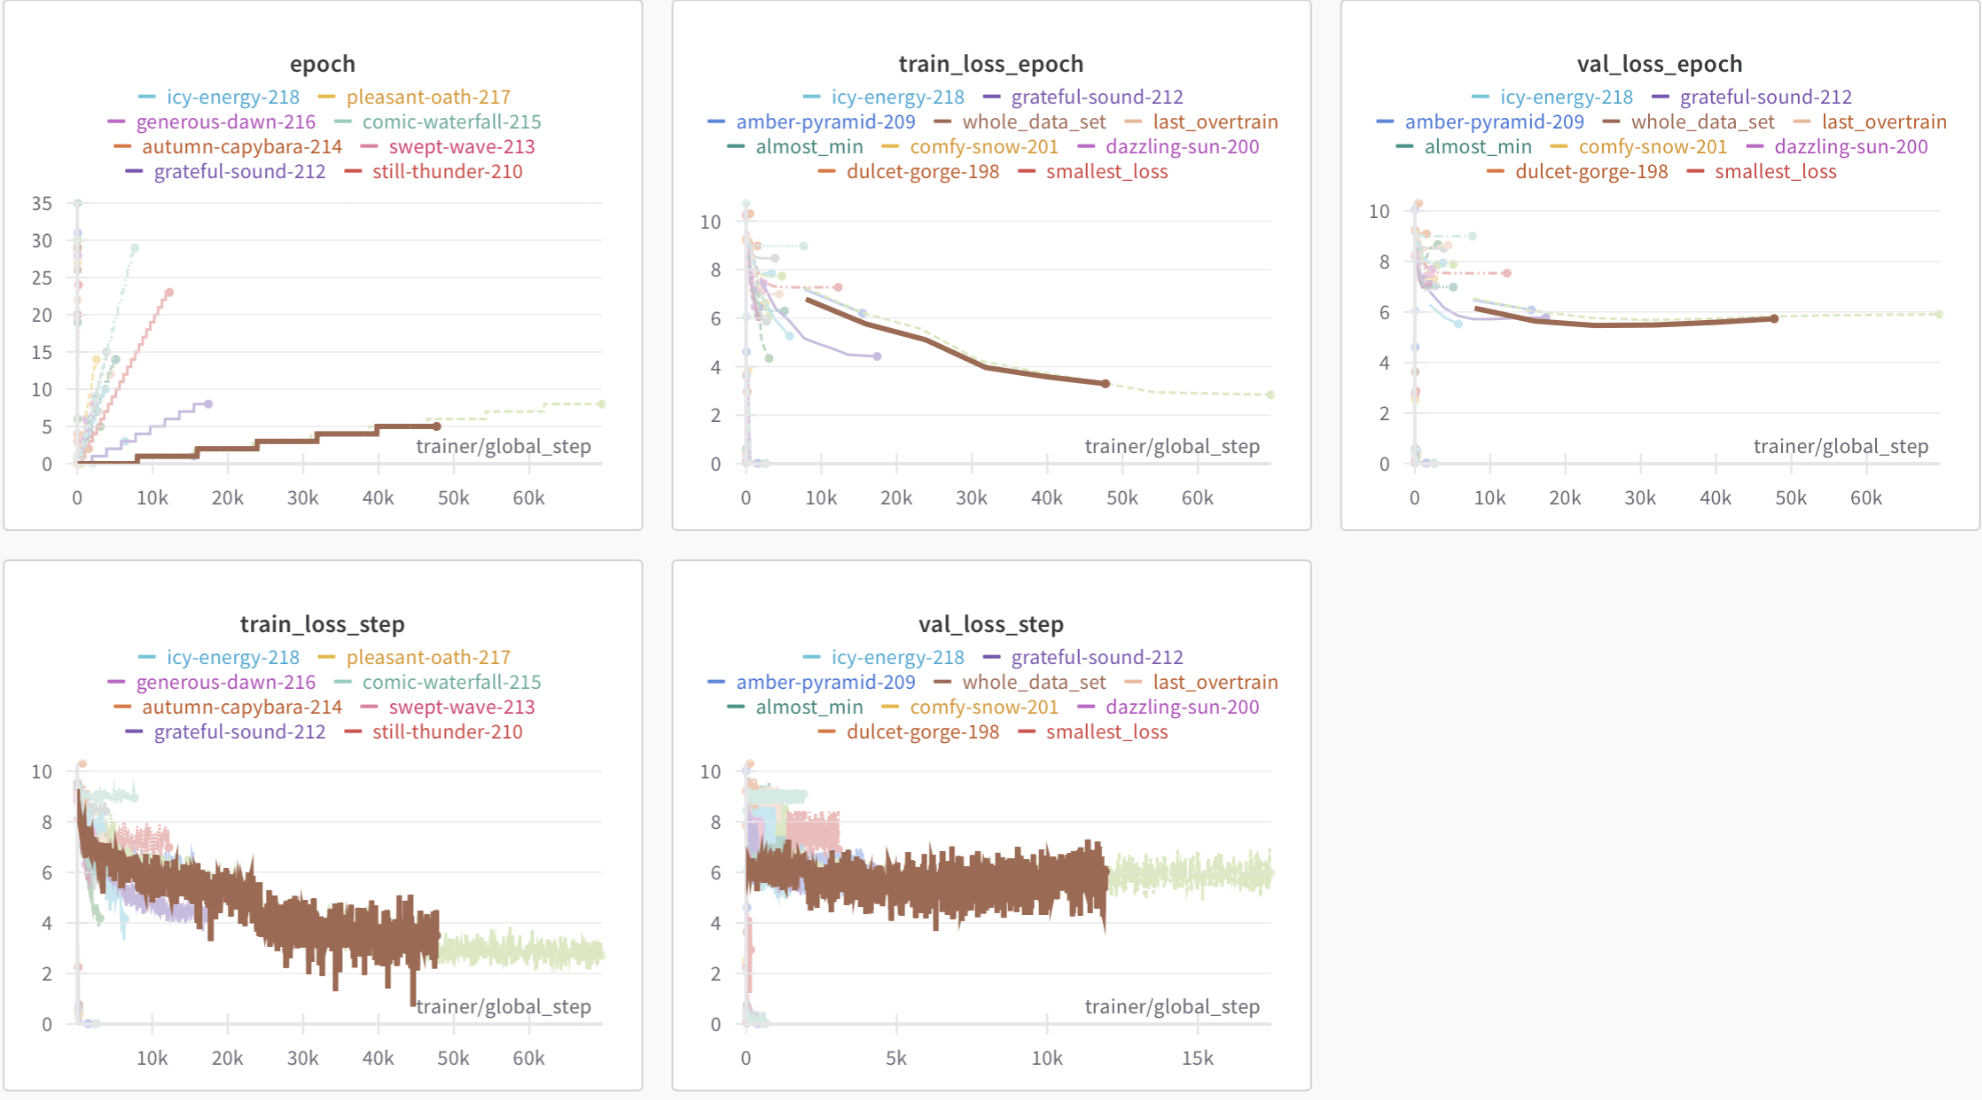
\includegraphics[width=\linewidth]{../assets/train.png}
    \caption{Training and validation losses in various experiments}
    \label{fig:synth}
\end{figure}

\section{Conclusions}
Although Mamba managed to generate novel samples, they weren't of high quality. This may be due to our models being unable to handle the complexities of virtuosic music. The model might be more suited for simpler datasets that do not contain such intricate musical scores.

\subsection{Future work}
While Mamba offers better performance than transformers, it comes at the cost of output quality. A promising direction for future research is to experiment with hybrid architectures that combine the strengths of both models. Examples of such architectures include \textbf{MambaFormer} \cite{mambaformer} and \textbf{Jamba} \cite{jamba}. It is also worth trying different datasets to see how Mamba handles them.

% \begin{thebibliography}{00}
%     \bibitem{b1} G. Eason, B. Noble, and I. N. Sneddon, ``On certain integrals of Lipschitz-Hankel type involving products of Bessel functions,'' Phil. Trans. Roy. Soc. London, vol. A247, pp. 529--551, April 1955.
%     \bibitem{b2} J. Clerk Maxwell, A Treatise on Electricity and Magnetism, 3rd ed., vol. 2. Oxford: Clarendon, 1892, pp.68--73.
%     \bibitem{b3} I. S. Jacobs and C. P. Bean, ``Fine particles, thin films and exchange anisotropy,'' in Magnetism, vol. III, G. T. Rado and H. Suhl, Eds. New York: Academic, 1963, pp. 271--350.
%     \bibitem{b4} K. Elissa, ``Title of paper if known,'' unpublished.
%     \bibitem{b5} R. Nicole, ``Title of paper with only first word capitalized,'' J. Name Stand. Abbrev., in press.
%     \bibitem{b6} Y. Yorozu, M. Hirano, K. Oka, and Y. Tagawa, ``Electron spectroscopy studies on magneto-optical media and plastic substrate interface,'' IEEE Transl. J. Magn. Japan, vol. 2, pp. 740--741, August 1987 [Digests 9th Annual Conf. Magnetics Japan, p. 301, 1982].
%     \bibitem{b7} M. Young, The Technical Writer's Handbook. Mill Valley, CA: University Science, 1989.
% \end{thebibliography}

\bibliographystyle{plain}
\bibliography{references}

\vspace{12pt}

\end{document}
